\clearpage
\section{Quantum Key Distribution Without Basis Switching}

\begin{refsection}

\begin{tcolorbox}	
\begin{tabular}{p{2.75cm} p{0.2cm} p{10.5cm}} 	
\textbf{Student Name}  &:&  Gonçalo Nunes\\
\textbf{Goal}          &:& Provide practical evidence of the employability of a coherent state quantum key distribution protocol based on simultaneous quadrature measurements.\\
\textbf{Directory}              &:& sdf/bpsk\_system
\end{tabular}
\end{tcolorbox}
Quantum key distribution (QKD) is a method to generate a cryptographic key between two distant parties, Alice and Bob, based on transmission of quantum states. After said transmission and respective measurement, Alice and Bob can then exchange classical messages through an insecure channel and, using the keys generated, perform post-processing to recover the messages.\\ 
In the first quantum key distribution schemes, single photons acted as information carriers (discrete variable regime). The practical implementation of said schemes was limited by the single photon generation and detection techniques. Hence the current interest in continuous variable (CV) quantum cryptography, which allows for higher key rates. Such protocols are carried out through the usage of squeezed and Einstein-Podolsky-Rosen entangled states, where the information is carried through the amplitude and phase quadratures of a coherent laser, and can  then  be  measured  by  the  receiver  using  homodyne detectors. The security of a CV-QKD relies on randomly switching the measurement basis (quadratures). In practice this implies a change of phase of a local oscillator beam which is difficult to achieve and constitutes a serious technical difficulty for the implementation of this type of cryptosystem, compromising its bandwidth.\\
Hence the pertinence of a QKD scheme that doesn't require for the change in mesurement basis. Such protocol was proposed in \cite{Weedbrook2004} and is called the simultaneous quadrature measurement or SQM Protocol, where both bases are measured simultaneously through double homodyne detection. It utilizes the quantum channel more effectively and achieves both higher secret key rates and bandwidths compared to orthodox CV-QKD protocols.
\subsection{Theoretical Analysis}
Recall the quadrature operators given from the annihilation, $\hat{a}$, and creation,$\hat{a}^\dagger$, operators by the expression:
\begin{equation}
\hat{X}^+\,=\,\hat{a}^\dagger\,+\,\hat{a}
\end{equation}
\begin{equation}
\hat{X}^-\,=\,i\left(\hat{a}^\dagger\,+\,\hat{a}\right)
\end{equation}
Here $X^+$ and $X^-$ correspond to the amplitude and phase of an electric field, respectively, and are analogous to position and momentum in classical physics. According to Heisenberg's uncertainty principle: $1\le V^+V^-$ Alice draws two random real numbers, $S^\pm$, following a Gaussian distribution with zero mean and variance of $V_S^\pm$. She prepares a state by displacing the amplitude and phase quadratures of a vacuum state by $S^+$ and $S^-$, respectively. The quadratures of sent states are the given by 
\begin{equation}
\hat{X}_A^\pm\,=\,S^\pm\,+\,\hat{X}_V^\pm
\end{equation}
Where $\hat{X}^\pm_V$ are the quadratures of the vacuum states. The resulting states has variances: $V_A^\pm\,=\,V_S^\pm+1$. The transmission of the state is done through a quantum channel with efficiency $\eta$ that inputs a noise of  $\hat{N}^\pm$. Bob simultaneously measures the amplitude and phase quadratures of the state using a 50/50 beam splitter. The state Bob receives is given by:\\
\begin{equation}
\hat{X}_B^\pm\,=\,\frac{1}{\sqrt{2}}\left(\sqrt{\eta}\hat{X}_A^\pm+\sqrt{\left(1-\eta\right)}\hat{X}_N^\pm+\hat{N}_B^\pm\right)
\end{equation}
And the variances of the state are:\\
\begin{equation}
V_B^\pm\,=\,\frac{1}{2}\left(\eta V_A^\pm+\left(1-\eta\right)V_N^\pm+1\right)
\end{equation}
Alice and Bob then test the channel transmission and bit error rate of their key by using a randomly chosen subset of their key to check for errors. If the rate of errors is within a certain limit they distill a secret key. In fact, the general protocol is very similar to an orthodox CV-QKD protocol,the only difference being that there's no need for Alice and Bob to differentiate which quadratures were measured.\\
The rate at which a secure key is given by:
\begin{equation}
\Delta I \geq \,\log_2\left(\frac{\left(\frac{\eta}{V_A}+\left(1-\eta\right)V_N\right)^{-1}+1}{\eta+\left(1-\eta\right)V_N+1}\right)
\end{equation}
Notice that, in order to generate a secret key, $\Delta \,I$ has to be greater than zero. $\Delta\,I$ has this nomenclature since it  represents the difference between the shared mutual information between Bob and Alice and Bob and Eve.\\
The expression implies that so long as the channel noise $V_N$ is not excessive, a secret key can be successfully generated between Alice and Bob, even in the limit of very small channel efficiency $\eta$. As the channel noise is reduced, or
efficiency increased, the rate at which a key can be established is enhanced. The expression tends towards an information rate of just over $5.5$ bits/symbol for perfect efficiency and a coherent vacuum noise.
%\begin{figure}[h]
%\centering
%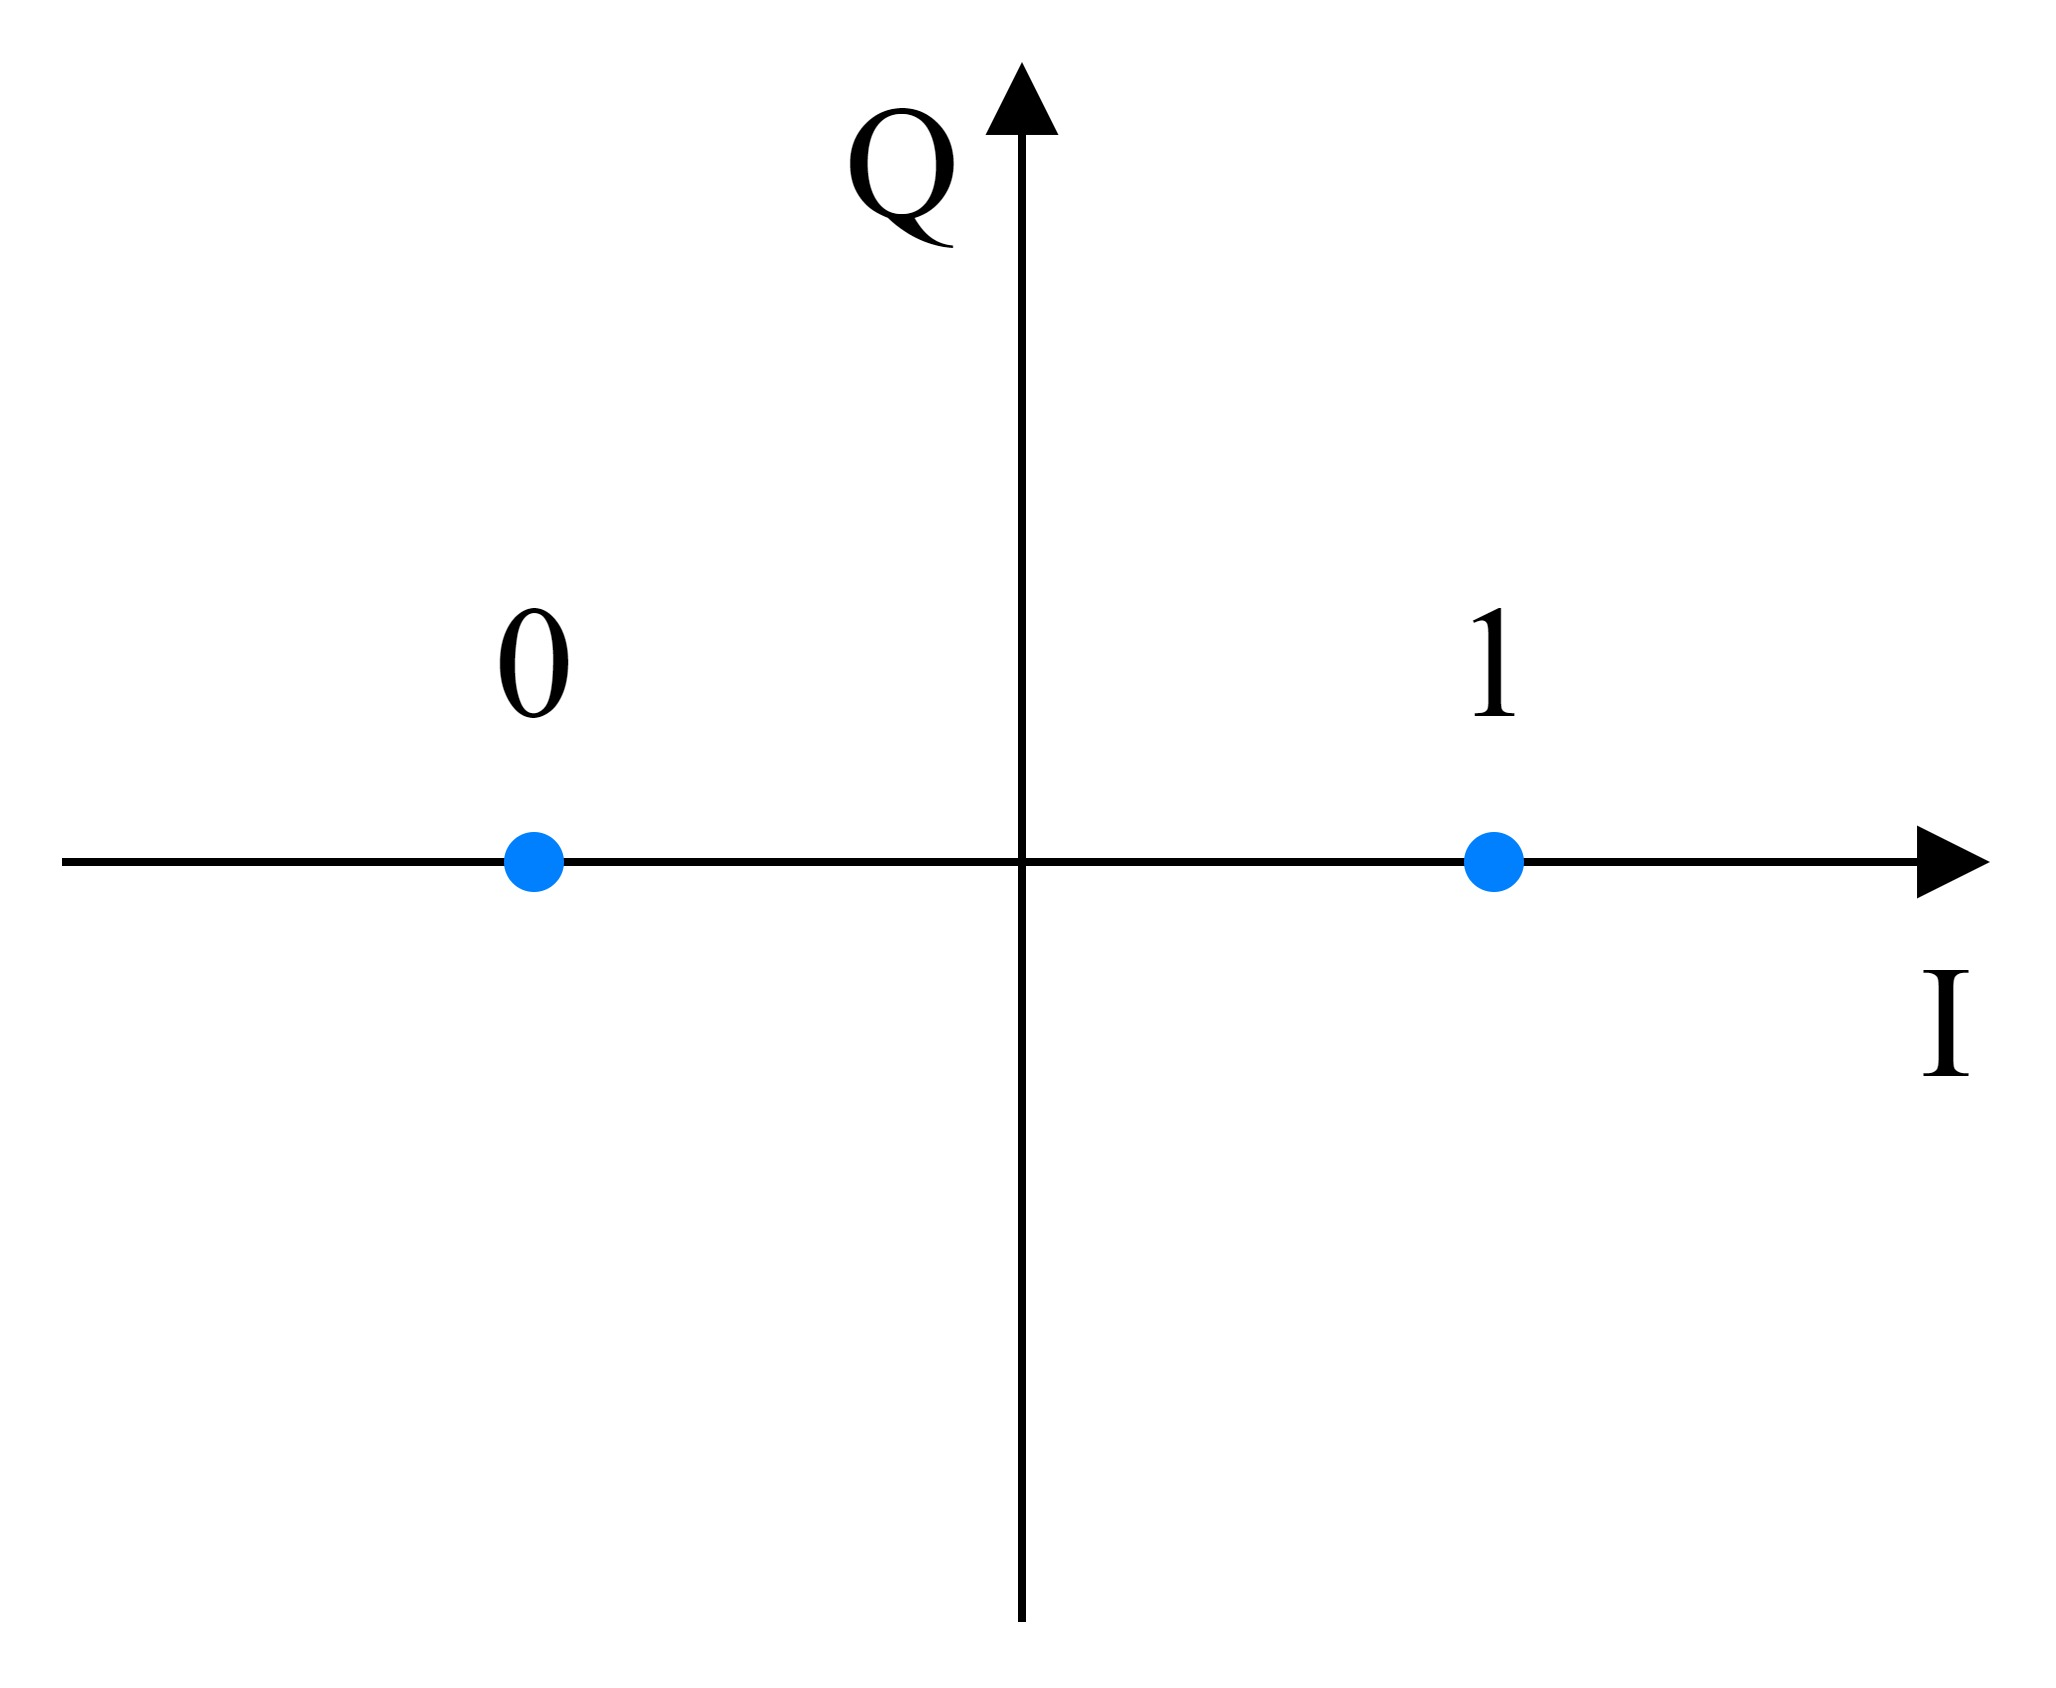
\includegraphics[width=.4\linewidth]{./sdf/bpsk_system/figures/bpskconstellation.jpg}
%\caption{BPSK symbol constellation.}
%\label{fig:BPSKConst}
%\end{figure}

% bibliographic references for the section ----------------------------
\clearpage
\printbibliography[heading=subbibliography]
\end{refsection}
\addcontentsline{toc}{subsection}{Bibliography}
\cleardoublepage
% --------------------------------------------------------------------- 